\documentclass[a4paper]{article}
\usepackage[english,spanish]{babel}
\usepackage[utf8]{inputenc}
\usepackage[T1]{fontenc}
\usepackage{verse}
\usepackage[noend]{algpseudocode}
\usepackage{listings}
%% Sets page size and margins
\usepackage[a4paper,top=3cm,bottom=3cm,left=3cm,right=3cm,marginparwidth=1.75cm]{geometry}
%% Useful packages
\usepackage{amssymb,amsmath,amsthm,amsfonts}
\usepackage{graphicx}
\usepackage[colorinlistoftodos]{todonotes}
\usepackage[colorlinks=true, allcolors=blue]{hyperref}

\newcommand{\verso}[1] {
\settowidth{\versewidth}{123456789012345678901234567890}%
\begin{minipage}[t]{\dimexpr\versewidth+1pt\relax}
\begin{verse}[\versewidth]
{\fontfamily{qzc}\selectfont\large
  #1
}
\end{verse}
\end{minipage}\bigskip
}

\title{Trabajo Práctico 1}
\author{Sebastián Cherny}



\begin{document}
\maketitle

1)\\
Explicación del código: Aprovechando que el parámetro de la función es una permutación, por lo que no puede tener elementos repetidos, creo un vector ($indices$) que en la posición $i$ diga en qué lugar se encuentra el número $i$ en la permutación, para $1 \leq i \leq n$. \\
Luego, en el vector $ans$ guardo en la posición $i$ la longitud de cadena consecutiva creciente más larga terminada en el número $i$, con una especie de programación dinámica: Sé que terminando en el número $1$ la cadena más larga tendrá longitud $1$, y para $i>1$, si el índice de $i-1$ es menor que el de $i$, el número $i$ se sumará a la cadena y su longitud valdrá $1$ más que la que termina en $i$, y si el índice de $i-1$ es mayor, entonces la longitud terminando en $i$ será $1$. El órden máximo será el mayor de los valores de $ans$.\\

2)\\
Para el riffle shuffle simplemente primero se elige un $K$ que será la cantidad de cartas del sub-mazo, mediante la distribución Binomial mencionada. Luego se eligen $K$ posiciones al azar del conjunto $\{1, 2, ..., n\}$ (sin reposición). Como $R$ los agarra en cualquier orden, ordeno este vector para lugar insertar en orden en las posiciones random seleccionadas, los números del $1$ al $K$. Y luego en las otras posiciones (if ans[i]==-1), inserto en orden también los números restantes, del $K+1$ al $n$.\\

3)\\
Al hacer un shuffle de una permutación ordenada de $n$ cartas, tomamos un sub-mazo de $k$ cartas y otro de $n-k$. Luego del shuffle, como las cartas de cada sub-mazo no cambian su orden relativo, habrá una cadena consecutiva creciente de al menos $k$ cartas (el primer sub-mazo en su orden inicial, y puede ser que cartas del segundo sub-mazo formen con el primer sub-mazo una cadena aún más larga), y otra cadena consecutiva creciente de al menos $n-k$ cartas.\\
Como el orden máximo es el mayor valor dentro de todas estas cadenas, luego de un shuffle será mayor o igual al máximo entre los valores $k$ y $n-k$, que como su suma da $n$, habrá exactamente uno mayor o igual a $\lceil \frac{n}{2}\rceil$ y exactamente uno menor o igual a $\lfloor \frac{n}{2}\rfloor$. Cuando $n=52$, el orden máximo luego de un shuffle no podrá ser menor a $26$.

Veamos qué pasa luego de dos shuffles:
Digamos que en el primer shuffle, el primer sub-mazo tuvo $k$ cartas y el segundo sub-mazo, $n-k$.
Sabemos que luego del shuffle las cartas de cada sub-mazo siguen ordenas como en la permutación inicial.

Luego, pensemos en las cartas únicamente del primer sub-mazo (para el segundo será análogo).

Digamos que de las $k$ cartas, $a$ quedan en el primer sub-mazo del segundo shuffle, y $k-a$ cartas quedan en el segundo sub-mazo.

Ahora, estas $a$ cartas siguen manteniendo su orden inicial, si bien pueden no estar todas juntas. Lo mismo pasa con las otras $k-a$ cartas, su orden relativo sigue manteniéndose como el inicial.
Luego, al hacer el shuffle, habrá una cadena consecutiva creciente de longitud al menos $a$, y otra de longitud al menos $k-a$. Por lo que el orden máximo será mayor o igual a $\lceil \frac{k}{2}\rceil$.

Análogamente, pensando en las cartas del segundo sub-mazo, el orden máximo será mayor o igual a $\lceil \frac{n-k}{2}\rceil$. Por lo que podemos concluir que luego de dos shuffles, el orden máximo será al menos $max(\lceil \frac{n-k}{2}\rceil, \lceil \frac{k}{2}\rceil) \geq \lceil \frac{\lceil \frac{n}{2}\rceil}{2} \rceil = \lceil \frac{n}{4}\rceil$

En el caso $n=52$, concluimos que luego de dos shuffles el orden máximo no puede ser menor a $13$. Si encontramos un ejemplo con su orden máximo igual a $13$, entonces esta será la mayor cota inferior.\\

Ejemplo:\\

Al inicio:\\

$1, 2, 3, ..., 50, 51, 52$\\

Shuffle 1: Cada sub-mazo contiene $26$ cartas, y los lugares elegidos para el primer sub-mazo son los ''segundos 13'' y los últimos $13$.\\

$27, 28, ..., 39, 1, 2, ..., 13, 40, 41, ..., 52, 14, 15, ..., 26$\\

Shuffle 2: Nuevamente cada sub-mazo contiene $26$ cartas, y los lugares elegidos son los mismos que antes:\\

$40, 41, ..., 52, 27, 28, ..., 39, 14, 15, ..., 26, 1, 2, ..., 13$\\

Se puede ver fácilmente que el orden máximo de esta última configuración es $13$ (tiene $4$ cadenas consecutivas crecientes de longitud $13$), y vimos que llegamos a ella a través de dos shuffles posibles.\\

Entonces como tenemos un ejemplo, la cota inferior es efectivamente $13$ para dos shuffles.\\

4)\\
Valor esperado de una corrida: 4.34\\
Desviación estándar de una corrida: 0.815\\

5)\\
Gráfico del orden máximo con su desviación estándar para $i$ shuffles ($1 \leq i \leq 20$) (simulado $100$ veces para cada $i$):\\

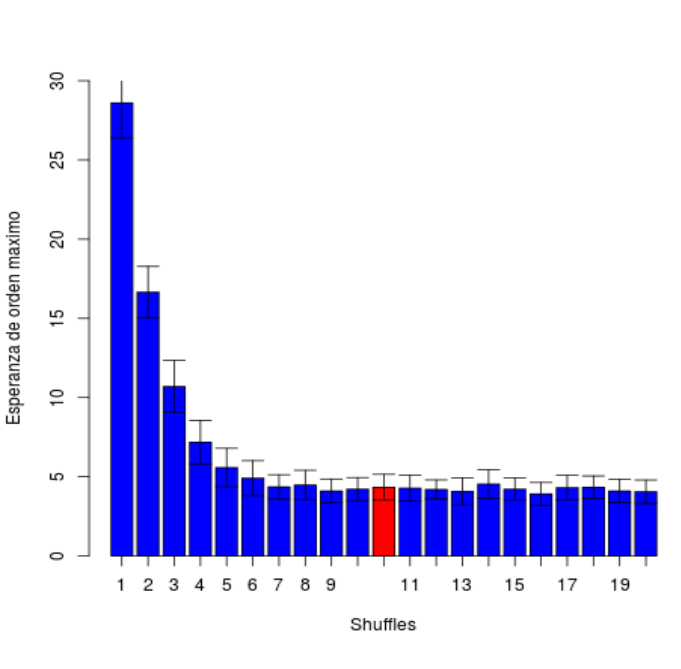
\includegraphics[width=12cm,height=9cm,keepaspectratio]{grafico.png}


La barra roja representa el valor (esperado y de desviación estándar) del orden máximo de una permutación al azar (lo obtenido en el punto $4$).\\

Se simularon hasta $20$ shuffles, realizando $100$ experimentos para cada cantidad de shuffles.\\

6)\\
Se ve cómo la esperanza comienza siendo bastante más grande que el valor en rojo y a partir de los 7 shuffles las barras son indistinguibles, incluyendo la roja. Teniendo en cuenta estos resultados, afirmo que mezclando 7 veces el mazo se aproxima a tomar una permutación al azar de las cartas.\\

\end{document}